%!TeX root = ./../Thesis.tex

%##########################################################
% Inhalt
%##########################################################
\chapter{Grundlagen}
Dieses Kapitel ist zur Vermittlung von technischen Grundlagen, um im Verlauf der Arbeit angewandte Technologien zu verstehen und umgesetzte Lösungsversuche nachvollziehen zu können. Dabei wird Fokus auf den SDLC, das Thema der LLMs sowie dem \textit{Prompt Engineering} gelegt. Da Unit-Tests einen wichtigen Bestandteil der Arbeit repräsentieren, werden Grundlagen zu diesen Tests geschaffen und der Bezug zur Programmiersprache Java hergestellt.

\section{Software Development Lifecycle}
Der SDLC ist ein Grundlagenzyklus, welcher innerhalb eines Softwareprojektes festgelegt und während der Bearbeitung des Projektes befolgt wird. \cite*{SoftwareDevelopmentLife} Dieser dient zur Verbesserung von Qualität und Entwicklungsprozess.
\begin{figure}[h]
    \centering
    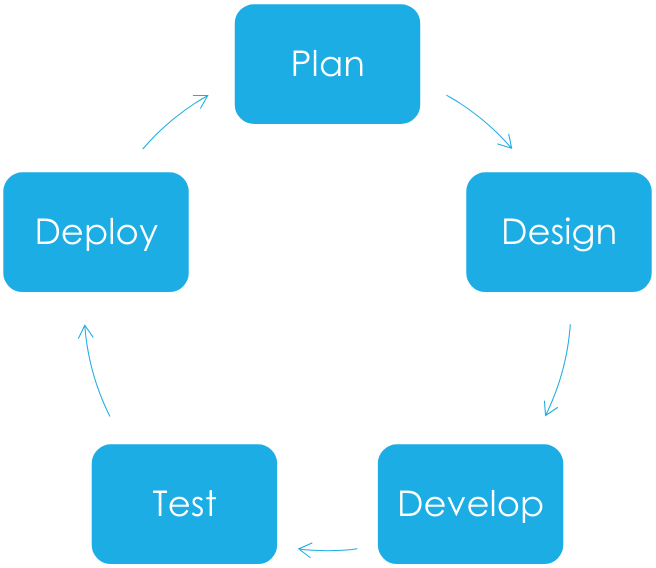
\includegraphics[scale=0.3]{Assets/Pictures/SDLC.png}
    \caption{Phasen eines SDLC - Quelle: \cite*{tikySoftwareDevelopmentLife}}
    \label{fig:sdlc}
\end{figure}
Ein typischer SDLC besteht aus 6 verschiedenen Phasen. [Abb. \ref{fig:sdlc}]\\\\
\textbf{Planung}\\[0.2cm]
Eine Planung erfolgt in der Regel durch eine neue Innovation, welche von einem Endnutzer oder Sponsor ausgeht. \cite*{tikySoftwareDevelopmentLife} Hierbei werden Projektumfang, Ziele sowie Anforderungen definiert. Dabei steht vor allem der Projektplan im Fokus, welcher Zeitrahmen und Ressourcen definiert. \cite*{hossainSoftwareDevelopmentLife2023}\\\\
\textbf{Entwurf}\\[0.2cm]
In der Entwurfsphase wird festgelegt, wie benötigte Softwarekomponenten zusammenwirken und eine Produktarchitektur definiert. Es kommt zum Entwerfen des \textit{User Interfaces} (engl. Benutzeroberfläche) mit Blick auf die \textit{User Experience} (engl. Benutzererfahrung). \cite*{hossainSoftwareDevelopmentLife2023}\\\\
\textbf{Entwicklung und Implementierung}\\[0.2cm]
Nach Abschluss aller vorher nötigen Phasen, beginnen Programmierer mit der Entwicklung und Implementation der Software bei Einhaltung aller festgelegten Anforderungen und entsprechend dem Architekturentwurf. \cite*{tikySoftwareDevelopmentLife} \\\\
\textbf{Testen}\\[0.2cm]
Das Testen der Software ist eine wichtige und essenzielle Phase, die während sowie nach der Entwicklung stattfindet. Hierbei kommt es zur Durchführung verschiedener Teststufen, einschließlich Unit-Tests, Integration Tests, System Tests und Benutzerakzeptanz Tests. Es werden Fehler identifiziert und behoben sowie Anforderungen aus vorherigen Phasen überprüft. \cite*{hossainSoftwareDevelopmentLife2023}\\\\
\textbf{Deployment und Wartung}\\[0.2cm]
Zum \textit{Deployment} gehört die Bereitstellung der Software in einer Staging-Umgebung. Diese wird vorausgesetzt um abschließende Tests durchzuführen und die Software zu validieren. Es werden Server und Datenbanken konfiguriert, sodass eine Produktionsumgebung vorbereitet wird. Nach erfolgreichen \textit{Rollout} (engl. ausrollen) der Software steht die Überwachung und Wartung der Produktionsumgebung im Fokus. \cite*{hossainSoftwareDevelopmentLife2023}\\\\
Insbesondere die Phase des Testens sollte als eine \textit{Sub stage} (engl. Unterstufe) jeder Phasen betrachtet werden, da ein Testen von Anforderungen, Implementation, Code sowie Deployment dauerhaft notwendig ist. Aufgrund dessen ist die Testphase besonders komplex und aufwändig, weshalb der Fokus ständig aufrechterhalten werden muss. \cite*{tikySoftwareDevelopmentLife}

\section{Large Language Models}
\subsection{Begriff und Einführung}
Hinter dem simplen Begriff \textit{Large Language Model} (engl. Großes Sprachmodell) steckt eine komplizierte Technologie mit großer Herkunftsgeschichte, welche eine Definition mehrerer Begrifflichkeiten im Feld der Künstlichen Intelligenz (kurz KI) vorraussetzt. Dadurch kann ein Grundverständnis geschaffen werden, um den Begriff LLM besser einordnen zu können. \cite{seemannKuenstlicheIntelligenzLarge} \\\\ Ein Hauptbestandteil der KI spielen \textbf{Künstliche Neuronale Netze} (kurz \acs{KNN}). 
Die Inspiration dieser Netze entstammt dem Neuronalen Netzwerk im Gehirn eines Menschen. \cite*{seemannKuenstlicheIntelligenzLarge} Das Ziel dabei ist, natürliche Organismen nachzubauen, und somit lernfähige Programme zu erzeugen. 
\begin{figure}[ht]
    \centering
    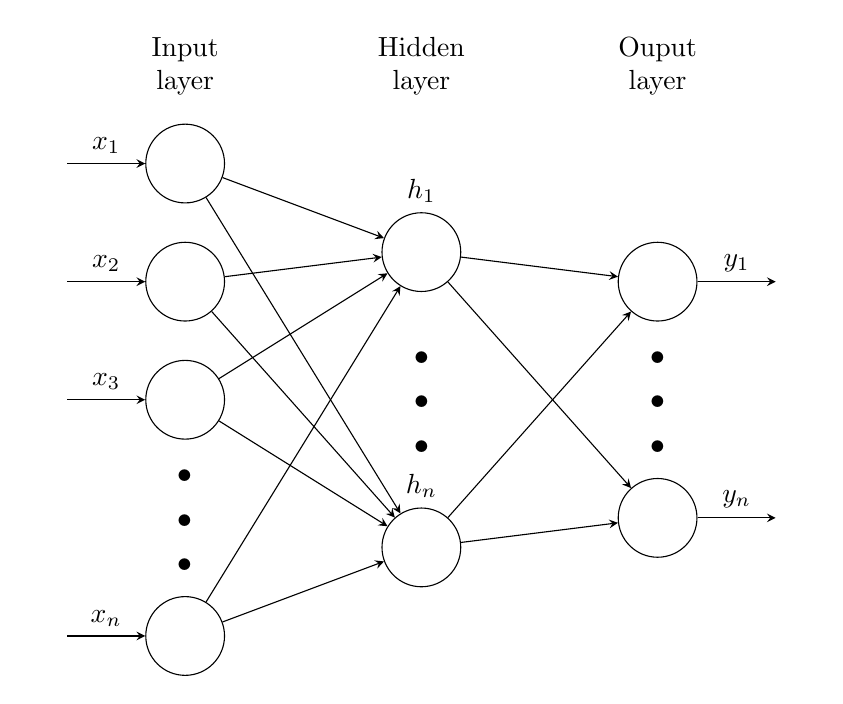
\begin{tikzpicture}[x=1.5cm, y=1.5cm, >=stealth]
        \tikzset{%
         every neuron/.style={
            circle,
            draw,
            minimum size=1cm},
        neuron missing/.style={
            draw=none, 
            scale=4,
            text height=0.333cm,
            execute at begin node=\color{black}$\vdots$},
        }
        
        \foreach \m/\l [count=\y] in {1,2,3,missing,4}
        {
            \node [every neuron/.try,neuron \m/.try] (input-\m) at (0,2.5-\y) {};
        }       
        \foreach \m [count=\y] in {1,missing,2}
            \node [every neuron/.try, neuron \m/.try ] (hidden-\m) at (2,2-\y*1.25) {};

        \foreach \m [count=\y] in {1,missing,2}
            \node [every neuron/.try, neuron \m/.try ] (output-\m) at (4,1.5-\y) {};

        \foreach \l [count=\i] in {1,2,3,n}
            \draw [<-] (input-\i) -- ++(-1,0)
                node [above, midway] {$x_\l$};

        \foreach \l [count=\i] in {1,n}
            \node [above] at (hidden-\i.north) {$h_\l$};

        \foreach \l [count=\i] in {1,n}
            \draw [->] (output-\i) -- ++(1,0)
                node [above, midway] {$y_\l$};

        \foreach \i in {1,...,4}
        \foreach \j in {1,...,2}
            \draw [->] (input-\i) -- (hidden-\j);

        \foreach \i in {1,...,2}
        \foreach \j in {1,...,2}
            \draw [->] (hidden-\i) -- (output-\j);

        \foreach \l [count=\x from 0] in {Input, Hidden, Ouput}
            \node [align=center, above] at (\x*2,2) {\l \\ layer};
    \end{tikzpicture}
    \caption{Grundlegender Aufbau eines KNN}
    \label{fig:knn}
\end{figure}
Der Aufbau eines solchen Netzes folgt dem Vorbild der Struktur des menschlichen Gehirns und besteht somit aus verbundenen künstlichen Nervenzellen (Neuronen), welche durch eine Eingabeschicht passende Ausgaben erzeugen. \cite*{morrKuNstlicheNeuronale} Unterschieden wird hier zwischen 3 verschiedenen Arten von Neuronen. Somit besteht ein Netz grundlegend aus Input-, Hidden- und Outputneuronen, zwischen denen eine gewichtete Verbindung herrschen kann. \cite*{NeuronaleNetzeEinfuhrung} [Abb. \ref{fig:knn}] Durch solch eine Struktur können KNN durch maschinelles Lernen mit großen Datenmengen trainiert werden und dadurch Fähigkeiten wie das Generieren von Texten erlernen. \cite*{seemannKuenstlicheIntelligenzLarge}\\\\ Ein weiteres Teilgebiet in der KI ist das \textbf{Natural Language Processing} (engl. Natürliche Sprachverarbeitung, kurz NLP). Hierbei liegt der Fokus auf der Interaktion zwischen Computern und menschlicher Sprache, in dem Algortihmen und Modelle ermöglichen, dass Computer die menschliche Sprache verstehen, interpretieren und auf sinnvolle Weise erzeugen können. \cite*{muruganNaturalLanguageProcessing2024} \\\\ Dies schafft die Grundlage eines \textbf{Large Language Models}, denn diese Modelle basieren auf KNN und sind spezialisiert auf die Natürliche Sprachverarbeitung. \cite*{seemannKuenstlicheIntelligenzLarge} Sie sind ausgelegt, um Beziehungen zwischen einzelnen Daten zu lernen und Sequenzen vorherzusagen. Insbesondere deswegen sind sie für die Generierung von Text in natürlicher Sprache geeignet, da sie die Fähigkeit besitzen Sprache aus großen Datensätzen von geschriebenen Texten im Internet sowie digitalisierten Büchern zu erlernen, um sich in neuartigen Situtationen angepasst verhalten zu können. \cite*{okerlundWhatChatterbox2022} \cite*{authorityofthehouseoflordsLargeLanguageModels} \\Ein \textit{pre-training} (engl. Vortraining) oder auch \textit{fine-tuning} (engl. Feinabstimmung) ist in vielen Fällen notwendig, um die Genauigkeit des Modells auf bestimmte Bereiche zu verbessern. \cite{HowLLMsWork} Um eine solche Genauigkeit zu gewährleisten, arbeiten Sprachmodelle mit dem Prinzip der \textit{Tokenisierung}. Im Rahmen dieses Vorverarbeitungsschritts erfolgt eine Zerlegung des Textes in Token, wobei diese aus Zeichen, Teilwörtern oder Symbolen bestehen können. \cite*{naveedComprehensiveOverviewLarge2024} \\ Grundlegend nehmen LLMs einen Prompt als Eingabe entgegen und generieren abhängig von gesetzten Parametern des Modells, sowie bisher erlernten Informationen, eine Ausgabe. Das vorhergesagte Wort ist das Ergebnis einer Wahrscheinlichkeitsverteilung des Modells, und wird solange mit der Sequenz verknüpft, bis sie endgültig ist. [Abb. \ref{fig:word}]
\begin{figure}[ht]
    \centering
    \tikzstyle{block} = [rectangle, draw, text width=5em, text centered, rounded corners, minimum height=3em, font=\small]
    \begin{tikzpicture}
        \tikzset{node distance = 0.75cm and 2.0cm}
        \node (n1) at (0,0) [rectangle, text width=5em, text centered, rounded corners, minimum height=3em]  {\colorbox{gray!25}{Es}};
        \node (n2) [block, above=of n1] {Wahrscheinlichkeitsverteilung};
        \node (n3) [block, above=of n2] {Sampling Strategy};
        \node (n4) [rectangle, text width=5em, text centered, rounded corners, minimum height=3em, above=of n3] {\colorbox{gray!25}{ist}};
        \node (n5) [rectangle, text width=5em, text centered, rounded corners, minimum height=3em, right=of n1] {\colorbox{gray!25}{Es ist}};
        \node (n6) [block, right=of n2] {Wahrscheinlichkeitsverteilung};
        \node (n7) [block, right=of n3] {Sampling Strategy};
        \node (n8) [rectangle, text width=5em, text centered, rounded corners, minimum height=3em, right=of n4] {\colorbox{gray!25}{ein}};
        \node (n9) [text width=5em, text centered, right=of n5] {\colorbox{gray!25}{Es ist ein}};
        \node (n10) [block, right=of n6] {Wahrscheinlichkeitsverteilung};
        \node (n11) [block, right=of n7] {Sampling Strategy};
        \node (n12) [rectangle, text width=5em, text centered, rounded corners, minimum height=3em, right=of n8] {\colorbox{gray!25}{schöner}};
        % Connectors
        \draw [->, thick] (n1) -- (n2);
        \draw [->, thick] (n2) -- (n3);
        \draw [->, thick] (n3) -- (n4);
        \draw [->, thick] ($(n4.east) - (0.35,0)$) -| ($(n4.east) + (1.0,0)$) |- ($(n5.west) - (1.0,0)$) -- (n5);
        \draw [->, thick] (n5) -- (n6);
        \draw [->, thick] (n6) -- (n7);
        \draw [->, thick] (n7) -- (n8);
        \draw [->, thick] ($(n8.east) - (0.35,0.0)$) -| ($(n8.east) + (1.0,0)$) |- ($(n9.west) - (1.0,0)$) -- (n9);
        \draw [->, thick] (n9) -- (n10);
        \draw [->, thick] (n10) -- (n11);
        \draw [->, thick] (n11) -- (n12);
        \draw [->, thick] ($(n12.east) + (-0.25,0)$) -- ($(n12.east) + (0.5,0)$);
        \draw [->, thick] ($(n1.east) - (0.35,0)$) -- (n5);
        \draw [->, thick] (n5) -- (n9);
    \end{tikzpicture}
    \caption{Wordgenerierung in LLMs}
    \label{fig:word}
\end{figure} 
Dabei können unterschiedliche Ergebnisse erzielt werden, welche abhängig von der \textit{sampling strategy} (engl. Stichprobenstrategie) sind. \cite*{cholletDeepLearningPython2018} Um auf die Qualität der Ergebnisse Einfluss zu nehmen, gibt es die Möglichkeit manuelle Parameter zu setzen. Darunter zählen z.B. \textit{max tokens} zum festlegen der maximalen Anzahl an Tokens, die generiert werden dürfen oder auch die \textit{temperature}, welche die Zufälligkeit von 0.0 (deterministisch) - 2.0 (extrem zufällig) regelt. Im Allgemeinen finden LLMs eine große Spannbreite an Anwendung, wie bspw. Textgenerierung, Vervollständigung und Zusammenfassung. \cite*{dhadukHowLargeLanguage2023}

\subsection{Modelle}


\section{Prompt Engineering}

\subsection{Prompt Techniken}

\subsection{LLM-Parameter und deren Einfluss}

\section{Unit Testing}


